\begin{acquis}
\begin{itemize}
\item lire et écrire des nombres décimaux en chiffres;
\item déterminer le chiffre des dizaines, des unités, des dixièmes, des centièmes… d'un nombre décimal;
\item déterminer le nombre de dizaines, d’unités, de dixièmes, de centièmes… d'un nombre décimal;
\item classer des nombres décimaux par ordre croissant et décroissant en utilisant les symboles < ou >;
\item placer des nombres décimaux sur une droite graduée et lire les abscisses de nombres décimaux placés sur une droite graduée;
\item encadrer un nombre décimal à une précision donnée;
\item déterminer l'arrondi d'un nombre décimal à une précision donnée;
\item utiliser le vocabulaire suivant : somme, différence, produit, quotient, terme, facteur, dividende, diviseur et reste;
\item soustraire, additionner et multiplier des nombres décimaux;
\item multiplier et diviser mentalement par 0,1; 0,01; 0,001; 10; 100; 1 000… des nombres décimaux et compléter les opérations à trous correspondantes;
\item faire une division décimale par un diviseur entier et non entier avec un résultat exact ou un résultat à une précision donnée ou un résultat arrondi;
\item convertir une durée en différentes unités de temps;
\item additionner et soustraire des durées sous la forme heures, minutes et secondes;
\item résoudre des problèmes dont la solution conduit à effectuer 2 ou 3 opérations successives parmi l’addition, la soustraction, la multiplication et la division de décimaux ou de durées;
\end{itemize}
\end{acquis}

%%%%%%%%%%%%%%%%%%%%%%%%%%%%%%%%%%%%%%%%%%%%%%%%%%%%%%%%%%%%%%%%%%%%%%%%%%%

\QCMautoevaluation{Pour chaque question, plusieurs réponses sont proposées. Déterminer celles qui sont correctes.} 

\begin{QCM}
  \begin{GroupeQCM} 
    \begin{exercice}
      Dix-huit millions huit cents s'écrit :
      \begin{ChoixQCM}{4}
      \item 18\,800\,000
      \item 18\,000\,800
      \item 18\,800
      \item 18\,008\,100
      \end{ChoixQCM}
\begin{corrige}
     \reponseQCM{b} 
   \end{corrige}
    \end{exercice}

    \begin{exercice}
      45 centaines est égal à :
      \begin{ChoixQCM}{4}
      \item 5 unités
      \item 450 dizaines
      \item 4 dizaines
      \item 45\,100
      \end{ChoixQCM}
      \begin{corrige}
     \reponseQCM{b}
   \end{corrige}
    \end{exercice}

    
    \begin{exercice}
      Un centième est :
      \begin{ChoixQCM}{4}
      \item plus grand qu'un dixième
      \item égal à dix millièmes
      \item plus petit qu'un millième
      \item égal à dix  dixièmes
      \end{ChoixQCM}
      \begin{corrige}
     \reponseQCM{b}
   \end{corrige}
    \end{exercice}


    \begin{exercice}
      Une écriture décimale de 456 centièmes est :
      \begin{ChoixQCM}{4}
      \item 456,100
      \item 456\,100
      \item 4,56
      \item 4\,560 millièmes
      \end{ChoixQCM}
      \begin{corrige}
     \reponseQCM{cd}
   \end{corrige}
    \end{exercice}


    \begin{exercice}
      Le nombre $5 + 0,4 + 0,007$ peut aussi s'écrire :
      \begin{ChoixQCM}{4}
      \item 547 millièmes
      \item 5,47
      \item 5,407
      \item 5\,047 millièmes
      \end{ChoixQCM}
      \begin{corrige}
     \reponseQCM{c}
   \end{corrige}
    \end{exercice}
 \end{GroupeQCM}  
\end{QCM}  
    
    
    
    
    
 \begin{QCM}
  \begin{GroupeQCM} 
       \begin{exercice}
      7 unités, 8 centièmes et 5 millièmes s'écrit :
      \begin{ChoixQCM}{4}
      \item 7,85
      \item 7,085
      \item 7,800\,500\,0
      \item 7,0085\,0
      \end{ChoixQCM}
      \begin{corrige}
     \reponseQCM{b}
   \end{corrige}
    \end{exercice}


     \begin{exercice}
      Un nombre compris entre 24,56 et 24,57 est par exemple...
      \begin{ChoixQCM}{4}
      \item 24\,568 millièmes
      \item 24,560\,7
      \item impossible, il n'y a pas de nombre compris entre 24,56 et 24,57
      \item $24 + 0,562$
      \end{ChoixQCM}
      \begin{corrige}
     \reponseQCM{abd}
   \end{corrige}
    \end{exercice}
    
     \begin{exercice}
      L'arrondi de 123,254 au dixième est...
      \begin{ChoixQCM}{4}
      \item 120
      \item 123,2
      \item 123,26
      \item 123,3
      \end{ChoixQCM}
      \begin{corrige}
     \reponseQCM{d}
   \end{corrige}
    \end{exercice}

     \begin{exercice}
      873,023 est ...
      \begin{ChoixQCM}{4}
      \item 1\,000 fois plus grand que 873\,230
      \item 100 fois plus petit que 87\,302,3
      \item 10\,000 fois plus grand que 0,087\,302\,3
      \item 10 fois plus petit que 87,302\,3
      \end{ChoixQCM}
      \begin{corrige}
     \reponseQCM{bc}
   \end{corrige}
    \end{exercice}
    
     \begin{exercice}
      $57,41 - 27,83 =$ ...
      \begin{ChoixQCM}{4}
      \item 30.42
      \item 30.58
      \item 29.58
      \item 19.58
      \end{ChoixQCM}
      \begin{corrige}
     \reponseQCM{c}
   \end{corrige}
    \end{exercice}


     \begin{exercice}
      $872,967 =$ ...
      \begin{ChoixQCM}{4}
      \item $87\,296,7 \div 100$
      \item $862,967 \cdot10$
      \item $87,296\,7 \cdot 10$
      \item $8,729\,67 \cdot 100$
      \end{ChoixQCM}
      \begin{corrige}
     \reponseQCM{acd}
   \end{corrige}
    \end{exercice}
    
     \begin{exercice}
      $78,23 \cdot 21,796 =$ ...
      \begin{ChoixQCM}{4}
      \item 170\,510,108
      \item 3\,705,101\,08
      \item 1\,705,101\,08
      \item 1\,800
      \end{ChoixQCM}
      \begin{corrige}
     \reponseQCM{c}
   \end{corrige}
    \end{exercice}
    
     \begin{exercice}
      $34,1 + 123,79$ se pose ...
      \begin{ChoixQCM}{4}
      \item 
      
      \includegraphics[width=1.5cm]{frac1}
      \item 
      
      \includegraphics[width=1.5cm]{frac2}
      \item 
      
      \includegraphics[width=1.7cm]{frac3}
      \item 
      
      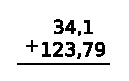
\includegraphics[width=1.5cm]{frac4}
      \end{ChoixQCM}
      \begin{corrige}
     \reponseQCM{ad}
   \end{corrige}
    \end{exercice}

    
     \begin{exercice}
      Une ficelle mesure 7,2 m. On la partage en 16.
      \begin{ChoixQCM}{4}
      \item Chaque bout mesure 1,152 m
      \item C'est impossible, $16 > 7,2$
      \item Chaque bout mesure environ 2,2 m
      \item Chaque bout mesure 45 cm
      \end{ChoixQCM}
      \begin{corrige}
     \reponseQCM{d}
   \end{corrige}
    \end{exercice}
    
    \begin{exercice}
      0,75 peut être la réponse du (ou des) problème(s) suivant(s) :
      \begin{ChoixQCM}{4}
      \item Avec 126 litres d'eau, on a rempli 168 bouteilles. Quelle est la contenance d'une bouteille ?
      \item Une baignoire peut contenir 223,24 L. On la remplit avec  222,49 L d'eau. Combien d'eau peut‑on encore verser ?
      \item Ahmed achète un bonbon à 0,27 CHF et un chewing‑gum à 0,58 CHF. Combien paye‑t‑il ?
      \item 125 CD de 6 mm d'épaisseur sont empilés. Quelle est la hauteur en mètre de la pile ?
      \end{ChoixQCM}
      \begin{corrige}
     \reponseQCM{abd}
   \end{corrige}
    \end{exercice}
    
    \begin{exercice}
      Henri court pendant 1 h 52 min. Il s'arrête à 10 h 07. Il est parti à...
      \begin{ChoixQCM}{4}
      \item 8 h 55
      \item 11 h 59
      \item 8 h 15
      \item 9 h 45
      \end{ChoixQCM}
      \begin{corrige}
     \reponseQCM{c}
   \end{corrige}
    \end{exercice}

\end{GroupeQCM}
\end{QCM}

  
